%d !TeX root = ../incremental_SS_Translation.tex
\chapter{Kalpasthāna 6: Rats and Rabies}
\label{mūṣikā}


\section{Introduction}

A notable macro-difference between the vulgate and the Nepalese
versions of the \SS\ is that this chapter and the next are reversed
in the vulgate.  In the Nepalese version, this is chapter six and the
chapter on antitoxic drumming is chapter seven.\footnote{See
    p.\,\pageref{kalpa-chapter-sequence} above.}  Jejjaṭa too read the
    chapters this way round, as reported by
    Ḍalhaṇa.\footnote{\label{dalhana-rat-sequence}\Dalhana{5.6.32}{582}: 
    \dev{jejjaṭastu 
    mūṣikakalpānantaraṃ dundubhisvanīyaṃ kalpaṃ paṭhati}.}

\subsection{Mouse or Rat?}

In 2004, Umberto Eco published a characteristically subtle and
enlightening book about translation entitled \emph{Mouse or
    Rat?}.\footcite{eco-2004} The title alluded to Eco's discussion of
the example of translating words for mice and rats across several
European languages that do not always distinguish these animals from
each other, or confuse them in other ways.  In Sanskrit too,
\emph{mūṣikā}, the subject and title of this chapter, does not
distinguish between mouse and rat.  The same is true for MIA and NIA
derivatives.\footcite[\#10258]{CDIAL}  It is hard to know quite how
to translate the term since “rodent” is too broad a term.  In what
follows, I have chosen “rat” for \emph{mūṣikā} in order to produce a
working translation of a text about an animal that is viewed as
potentially toxic and threatening.  ``Mouse'' does not have quite
these connotations for a contemporary English
speaker.\footnote{\citeauthor{bhis-1907} made the same choice
    \pvolcite{2}[728--736]{bhis-1907}.}

The rodents that may be described as mice or rats in contemporary
South Asia and that are especially associated with the spread of
disease include the house or black rat (\emph{Rattus rattus}, L.),
the brown rat (\emph{R.\ norvegicus}, Berkenhout), the house mouse
(\emph{Mus musculus}, L.) and bandicoots
(\emph{Bandicota}).\footcite[194]{bia} Also present in SA are the
Indian desert gerbille (\emph{Meriones hurrianae}, Jerdon), the
Indian gerbille (\emph{Tatera indica}, Hardwicke), the spiny field
mouse (\emph{Mus platythrix}, Bennett), the Indian field mouse
(\emph{M. booduga}, Gray), the Metad (\emph{Millardia meltada},
Gray), the Indian bush rat (\emph{Golunda ellioti}, Gray), the
longtailed tree mouse (\emph{Vandeleuria oleracea}, Bennett), Royle's
vole (\emph{Aticola roylei}, Gray), the Indian mole-rat
(\emph{Bandicota bengalensis}, Gray \& Hardwicke),\footnote{“Recent
    studies\ldots show that the mole-rat forms 98\% of the total rodent
    population of Calcutta,” \cite[206]{bia}.} the bandicoot rat
    (\emph{B. indica}, Bechstein), the shorttailed bandicoot
    (\emph{Nesokia indica}, Gray \& Hardwicke), the whitetailed wood rat
    (\emph{Madromys blanfordi}, Thomas), the bay bamboo rat
    (\emph{Cannomys badius}, Hodgson), and other similar
    rodents.\footnote{\cite[ill.\ plates \,45, 46 \emph{et passim}]{bia}.
        See also \cite[passim]{meno-2014}.} However, plausibly matching
        these creatures to the Sanskrit names listed in this chapter is hard
        to impossible.\footnote{Mouse-words that we do not see in this
            chapter include the \emph{kirika, giri, girikā} group
            \pvolcite{1}[353, 488, 566]{EWA}.}  Almost no works engage directly
            with the representation or identity of rodents in pre-modern
            India.\footnote{One of the few is \cite[ch.\,3]{geer-2008}.}


\subsubsection{Rabies}

Passages 43\,ff. (p.\,\pageref{rabies}) describe rabies fairly unambiguously, 
including the symptoms of hydrophobia.\footnote{For a short historical 
bibliography on rabies, see \volcite{IB}[400, note 
163]{meul-hist}.}  As Meulenbeld noted, the idea that the bite-victim displays the 
behaviours of the creature that bit them is not unique to South 
Asia.\fvolcite{IB}[400, note 164]{meul-hist}


A sympathetic description was given in the seventeenth century by
Emperor Jahangir, in his \emph{Memoirs} (\emph{Tuzuk-e-Jahangiri}),
of the death of two of his elephants resulting from the bites of a
mad dog.\footcites[132--134]{alvi-1968}[145--146]{thac-1999}


\subsection{Literature}

A brief survey of this chapter's contents and reference to the
limited existing research on it to 2002 was provided by
Meulenbeld.\footnote{\volcite{IA}[295--296]{meul-hist}. In addition
    to the translations mentioned by \tvolcite{IB}[314--315]{meul-hist},
    a translation of this chapter was included in
    \volcite{3}[67--77]{shar-1999}. \citet{sekh-2023} omitted mention of
    this type of poisoning, although he discussed rabies, a subsection of
    this chapter.}
    

 \citeauthor{chev-1870} provided a characteristically vivid
nineteenth-century discussion of injuries inflicted by wild animals,
including details of those killed by wolves, tigers, dogs, jackals
and other animals, and in his classic survey of the diseases of
India, he discussed rabies
specifically.\footcites[359--368]{chev-1870} [426--440]{chev-1886}
The experiments with cannabis anesthesia conducted by William
O'Shaughenessy in Calcutta earlier in the nineteenth century were
largely aimed at palliative care for rabies
patients, an incurable, lethal disease.\footcite[50--55]{wuja-cann}


A rich description of Indian rodents is available by \citeauthor{bia},
including several useful illustrations.\footcite[ch.\,13,
esp.\,205--215]{bia} Unfortunately, \citeauthor{bia} rarely provided 
Indian-language names for the animals he described.

In Sanskrit literature, the \emph{Arthaśāstra} referred to the problem of rats 
more than once.  For example, to rid a country of the threat of rats, 
\begin{quote}    
    When there is a danger from rats, cats and mongooses should be
released. If these are captured or killed, the fine is 12 Paṇas,
as also for not keeping dogs confined, except in the case of
foresters. He should strew grains smeared with the milk of the
Snuhi-plant or mixed with secret compounds. Or, he should
institute a rat tax; or thaumaturgic ascetics should perform a
pacificatory rite. On the days of the moon’s change \ldots,
moreover, he should have rites of rat worship carried
out.\footnote{\emph{Arthaśāstra} 4.3.20--26, tr.\ \cite[230]{oliv-2013}.}
\end{quote}




\newpage

\section{Translation}

\begin{translation}
    
    \item[1] 
    
Now I shall explain the \se{kalpa}{procedure} relating to 
\se{mūṣikā}{rats}.\footnote{The word \dev{mūṣikā} does not distinguish 
between rats and mice.  See Introduction above.}
    
    \item[3] 
    
    Learn concisely about aforementioned eighteen kinds of rats that have 
    poison in their semen, according to their names, characteristics and the 
    herbal treatments.\footnote{Rats with poisonous semen were mentioned 
    in \Su{5.3.5}{567} (see p.\,\pageref{sukravisa} above).}
    
\subsection{The types of rat}

    \item[4--6]
    
    The eighteen rats are traditionally called,\footnote{\Dalhana{5.6.4}{582} 
    gave no 
    comment on any of these names.  The identifications are 
    mostly guesswork and sometimes whimsical.  The glossary gives lexical 
    discussion of individual names.}
\begin{multicols}{2}
    \begin{enumerate}
        \item \Gls{lālana},
        \item \Gls{putraka},
        \item \Gls{kṛṣṇa},
        \item \diff{\Gls{vasira-animal}},
        \item \Gls{cikkira}, % Beng Cika = chuchundara, regional
        \item \Gls{chuchundara} % Bengali house shrew Suncus murinus       
        \item \Gls{arala-animal},% hapax legomenon, Dravidian
\footnote{The word \dev{arala} is a hapax legomenon and has not 
previously been identified as a lexeme because it did not appear in earlier 
editions of the \SS.  It is a loan-word from Dravidian (see glossary).}        
        \item \Gls{kaṣāyadaśana},
        \item \Gls{kuliṅga},
        \item \Gls{ajita},
        \item \Gls{capala},
        \item \Gls{kapila-animal},
        \item the one called \Gls{kokila-animal} and 
        \item \Gls{aruṇa},
        \item the large black \gls{unduru}, 
        \item \Gls{śveta-animal}, together with the
        \item the large \Gls{kapila-animal},
        \item and the \Gls{kapota-animal}-like rat.\footnote{The Nepalese list has 
        \dev{vasira} (\Gls{vasira-animal}) for the 
        vulgate's \dev{haṃsira}.  The terms \dev{ākhu}, \dev{mūṣikā} and 
        \dev{unduru} are here used as generic names of rat/mouse rodents.}
\end{enumerate}
    \end{multicols}
\medskip
    
\item[7]

If a part of the body has their sperm fall on it or if they touch it
with their nails or teeth, etc., that have been touched by sperm,
then the blood is corrupted.\footnote{\label{alambayana2}On this,
    \Dalhana{5.7.7}{582} quoted an authority called Ālambāyana who
    elaborated on this subject (see \volcite{IA}[658]{meul-hist} for
    references to this author of a lost treatise on toxicology). Ḍalhaṇa
    also cited Ālambāyana elsewhere on the topics of insects and spiders
    \pvolcite{IB}[722, note 5]{meul-hist}. See also the \AS's assertion 
    that Ālambāyana was responsible for the doctrine of \sepl{vega}{toxic 
    pulse}, p.\,\pageref{alambayana1} above.
    
Ālambāyana, who was already known as “the famous soul of compassion”
in the \emph{Mahābhārata} (13.18.4), was also known in Buddhist
literature. Book 22, tale 543 of the Jātakas includes mention of
an Ālambāyana who claimed to be a doctor and specialist in
snakebite poisons: \emph{nāhaṃ dijādhipo homi, na diṭṭho garuḷo
mayā, āsīvisena vitto ti vejjo maṃ brāhmaṇaṃ vidū ti 793}
(\volcite{6}[181]{faus-1877}, tr.\  \volcite{6}[95]{cowe-1895}).
In the same tale, there is a herbal “Ālambāyana mantra” given to
an ascetic by a Garuḍa who has just caught and eaten a Nāga, thus
invoking the Garuḍa-snake-poison motif
\pvolcite{6}[93--94]{cowe-1895}.  The Jātakas were translated
into Chinese in the third century \CE.
    
    %
    %    Pāli text: \volcite{6}[177\,ff.]{faus-1877}
    %
    %    \pvolcite{6}[93--94, 95--98, 99]{cowe-1895}
    %
    See further discussion by \citet[33--34]{slou-2016}, who calls
    the mantra “Alampāyana,” adopting the reading of the Burmese MS
    Bd against the Fausbøll's critical reading  “Ālambāyana” 
    \pvolcite[see]{2 \& 3}[ Preliminary remarks 3 and 7]{faus-1877}.}
    
\item[8--10ab]

% TODO: \usepackage{graphicx} required
\begin{figure}
    \centering
    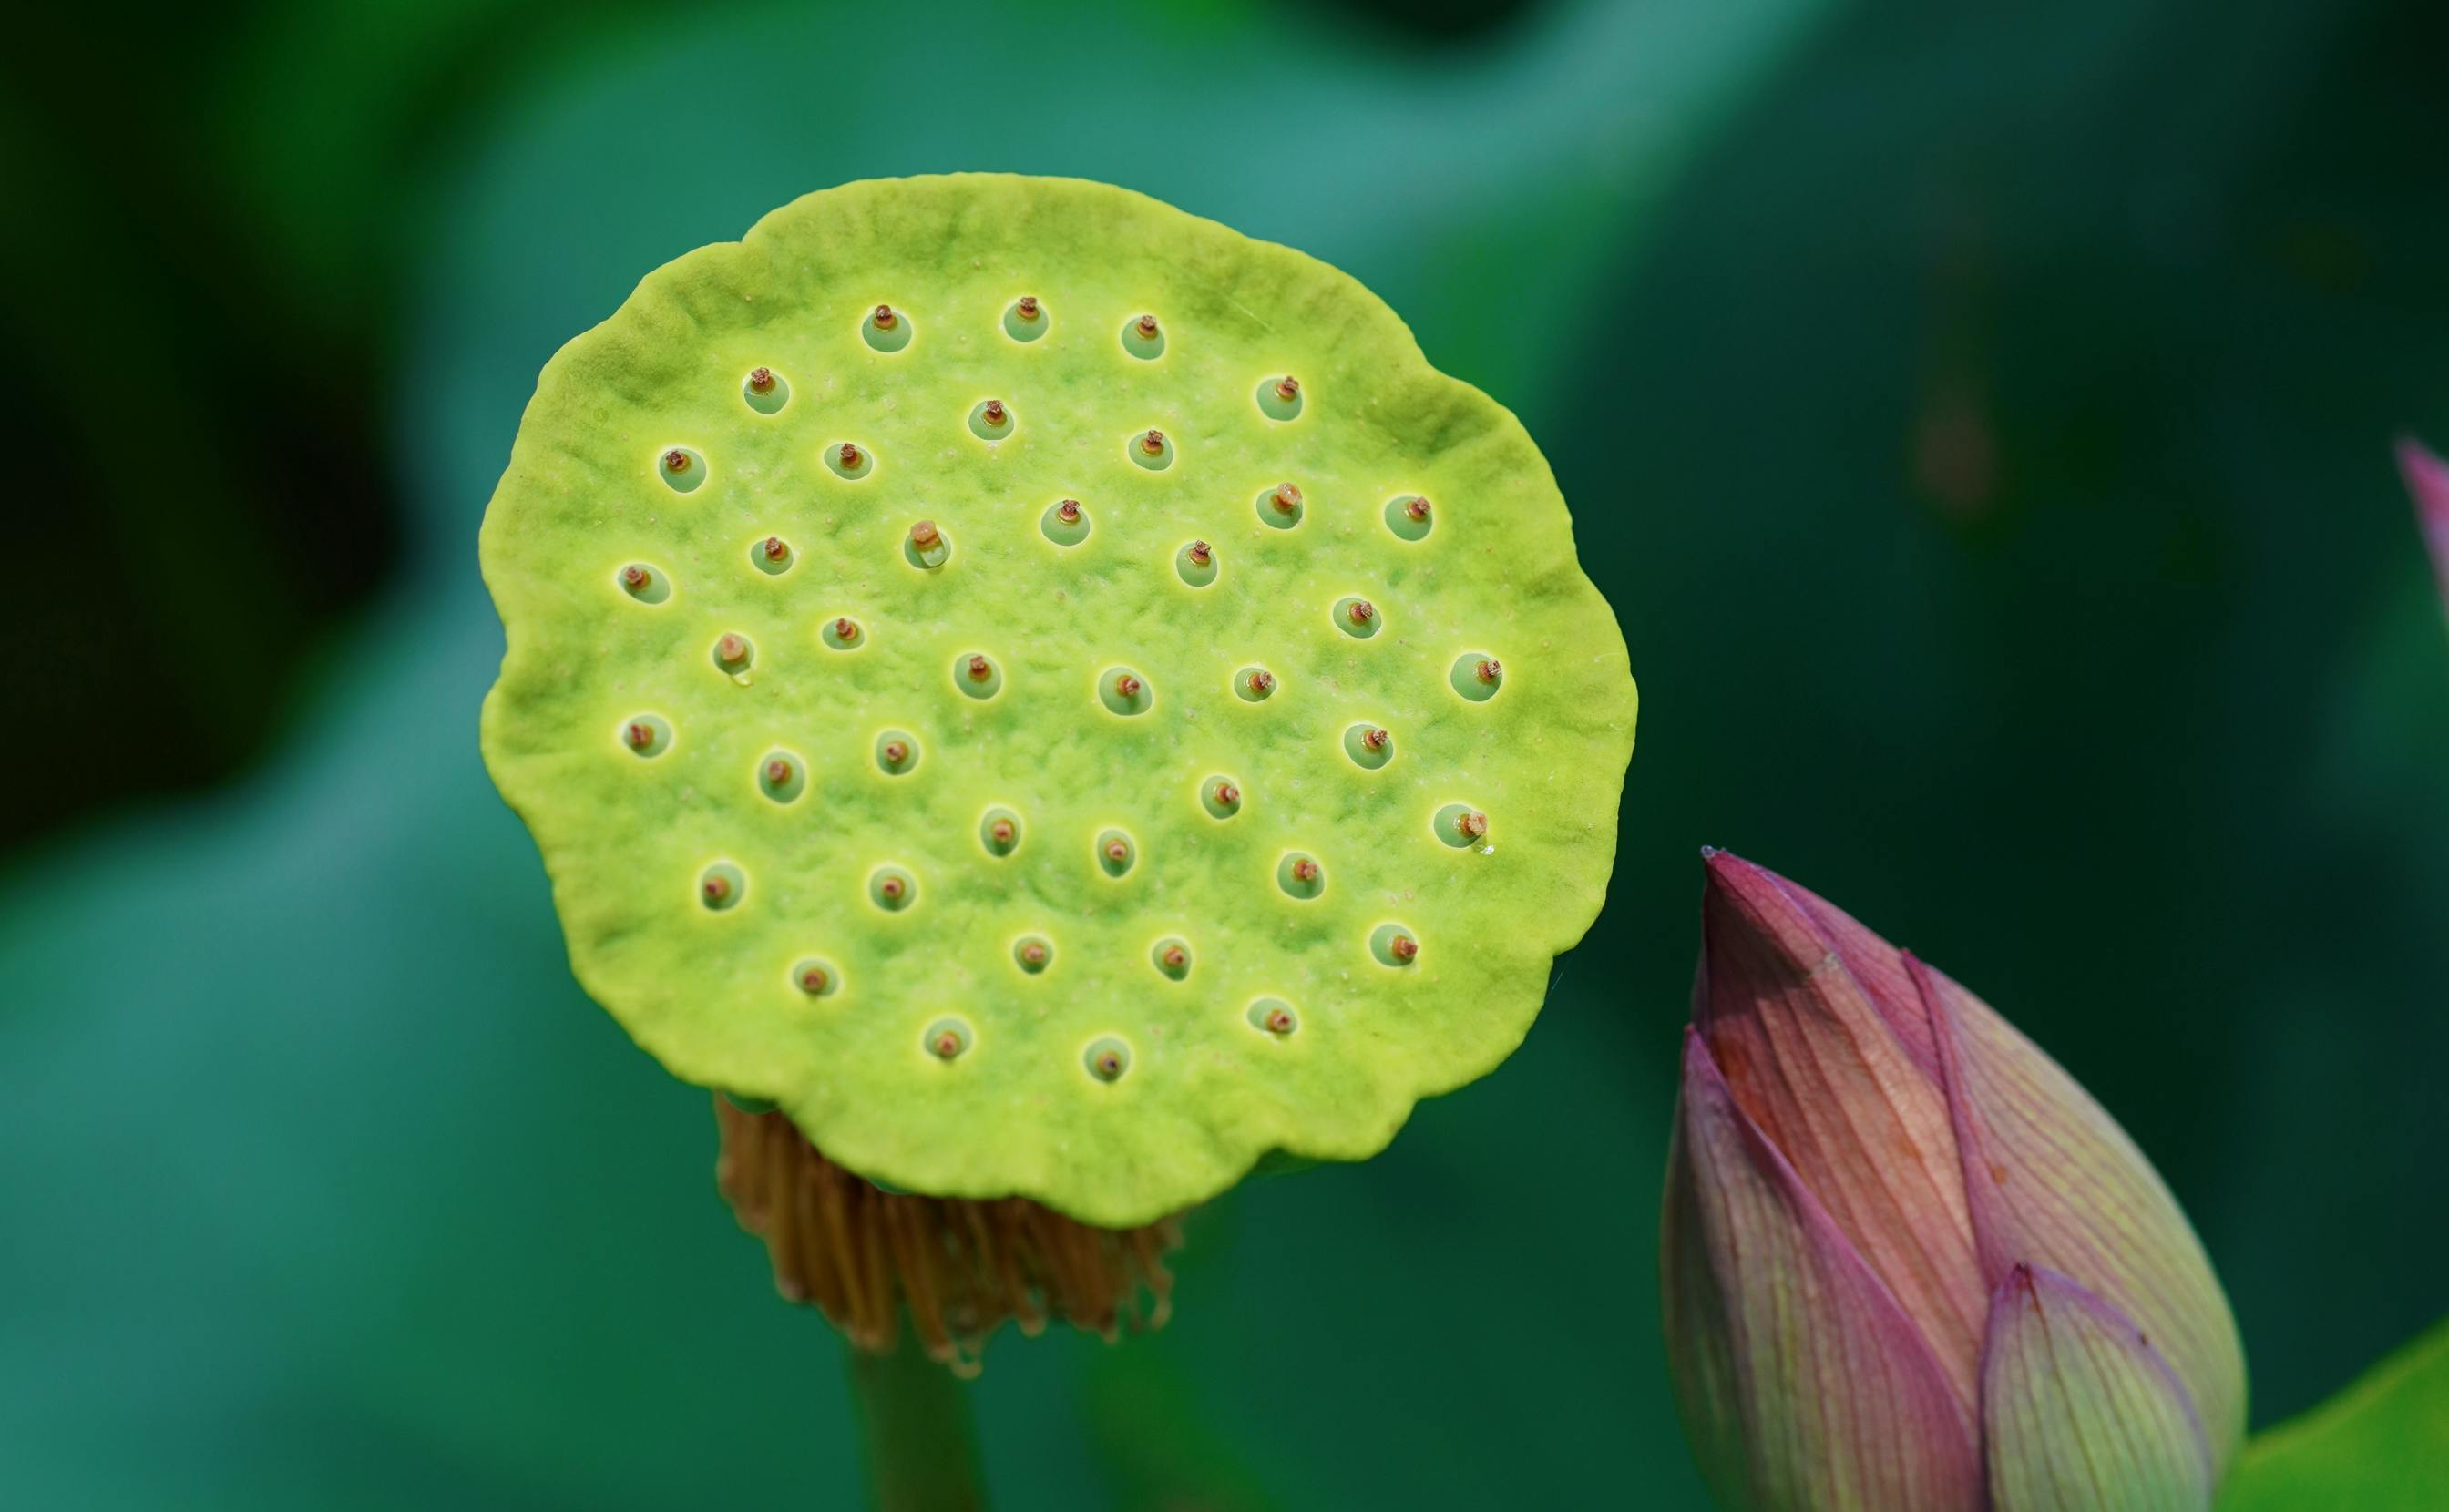
\includegraphics[width=0.7\linewidth]{media/lotusbud}
    \caption{“\,`Little ears' (\emph{karṇika}) look like the seed pod in the middle 
    of a lotus --- \Dalhana{5.7.8}{582}.” Credit: Pexels, CC license.}
    \label{fig:lotusbud}
\end{figure}

It happens that there are \se{granthi}{lumps}, swellings,
\se{karṇika}{small ear-like growths} and rings, accumulations of
severe \diff{\se{piṭaka}{blisters}}, \se{visarpa}{spreading rashes}
and \se{kiṭibha}{dark, rough patches of
    skin}.\footnote{\label{karṇika}“Little ears” was strikingly described
    by \Dalhana{5.7.8}{582} as looking like the seed pod in the middle of
    a lotus (\dev{kamalamadhyabījakośākṛtiḥ}), a graphic image (see also
    \Dalhana{5.8.136}{594}).  See Figure~\ref{fig:lotusbud}.  Perhaps similar to 
    hypergranulation. 
    %    lumps of
    % flesh
    % that look like
    %    the ears of a lotus (\dev{karṇikā māṃsakandī,
    %    padmakarṇikākāratvātkarṇkikā bhaṇyate}).
    The Nepalese version has \dev{piṭaka} “blisters” for the
    vulgate's \dev{pīḍaka} “boils” (itself perhaps a typo for
    \dev{piḍaka}).  \dev{kiṭibha} “dark rash” was described by
    \Dalhana{1.11.7}{46} as a kind of \dev{kuṣṭha}, which is
    variously a skin disease of pallor, leucoderma, or leprosy
    \citep{emme-1984}. But it was described in the \CS\ as being dark
    and as rough as a callous to the touch (\Ca{6.7.21cd--22ab}{451})
    \pvolcite{1}[208]{josi-maha}.}  There are severe conditions such
    as pain in the joints, pain, fever, fainting, weakness, loss of
    appetite, exhaustion, nausea and
    horripilation.\footnote{\dev{parvabheda} “pain in the joints” was
        glossed by \Dalhana{5.7.9}{582} as “spots on the joints”
        (\dev{sandheḥ sphoṭaḥ}).  This seems unlikely, since symptoms on
        the surface of the body were described in the previous verse, and
        also because of the obvious etymological meaning of the
        compound.}
        

This is a concise description of the appearance of someone who has been 
bitten.  Now listen to a longer version. 

\subsection{Detailed symptoms}

\begin{itemize}
\item[10cd--11ab]

The \Gls{lālana} causes a flow of saliva, vomiting and hiccups.  For that, one 
should lick a paste of \gls{taṇḍulīyaka} with honey. 

\item [11cd--12]

The \Gls{putraka} causes the limbs to droop and creates a pale
\diff{beauty},\footnote{The expression \dev{-valgu} “beauty” in the
    Nepalese MSS, for the vulgate's simpler \dev{-varṇa} “complexion,” is
    unusual.} and the body is heaped with lumps like the young of a
    rat.\footnote{The grammar here is very loose. \dev{śiśur} cannot
        stand outside the compound, which should read
        \dev{mūṣikaśisusaṃsthitaiḥ}.  The vulgate text has the simpler and
        grammatical \dev{ākhuśāvakasannibhaiḥ} “resembling the offspring of a
        rat.”}  One should lick \gls{śirīṣa}, \gls{iṅgudi} and \gls{patra}
        with honey.\footnote{\Dalhana{5.7.11-12}{582} here cited a passage 
        by
            an unknown author called Nāgārjuna, about the visible symptoms of a
            bite by this kind of rat (cf.\ \cite[45--46]{shar-1982},
            \volcite{IB}[497, note 100]{meul-hist}) as well as variant readings
            by Gayadāsa and Jejjaṭa on the exact formulation of the lickable
            medication.}

\item [13]

The \Gls{kṛṣṇa} causes one to vomit blood, especially when the
weather is bad.  One should drink \gls{śirīṣa} and \gls{patra},  
with \gls{kuṣṭha} and \gls{elā}, with the 
\gls{kiṃśuka} ashes.\footnote{\Dalhana{5.7.13}{583} explained “with the 
ashes of \gls{kiṃśuka}” as “water with the ashes of \gls{kiṃśuka}.”}

\item [14]

The \Gls{vasira-animal} causes a person have a revulsion for food, to yawn,
and makes their body-hair \diff{leprous}.\footnote{The qualifier
    \dev{kuṣṭhatā} (\dev{romṇāṃ}) is odd; the vulgate's \dev{harṣaṇa}
    “horripilation” reads more easily. \dev{kuṣṭha} has a lesser-known
    meaning “prominent part, mouth or opening” which might perhaps be
    considered here, though it is hard to see how.}  They should drink
    items like \gls{āragvadha} and be quickly made to vomit.

\item[15]

The \Gls{cikkira} causes headache, swelling, hiccups and nausea.  One
should have thorough emesis using
decoctions\sse{kvātha}{decoction} of \gls{jālinī}, and he should drink
the juice of \gls{aṅkolla}.

\item[16cd--ab]

The \Gls{chuchundara} causes constipation, paralysis of the neck, and
\se{vijṛmbhikā}{gasping}.\footnote{\dev{vijṛmbhikā} is one of the
    eighty wind diseases listed in the \emph{Kāśyapasaṃhitā} and glossed
    by Hemarājaśarman as “yawning” (Hindī \dev{jaṃbhāī},
    \Ka{1.27.19--28}{41--42}). However, in the \CS\ it is a term for one
    of the disorders of an improperly treated post-partum umbilical cord
    (glossed by Ḍalhaṇa as \dev{muhurmuhurvṛddhimatī} “growing larger
    moment by moment,” \Ca{4.8.45}{348--349}) and translated by
    \tvolcite{1}[480]{shar-1994} as “umbilical hernia.”
    Cf.\,\volcite{1}[756]{josi-maha}.} %
    In this case, one should administer a caustic made of
    \gls{yavanāla} and \gls{ārṣabhī} as well as the two
    \glspl{bṛhatī}.\footnote{Note that half-verses 16cd and 16ab are
        reversed compared to the vulgate edition.  This makes the caustic
        a remedy for the bite of the \Gls{chuchundara}, while the
        earlier \gls{jālinī} remedy is for the \Gls{cikkira}, which makes
        betters sense.
        
        The vulgate has text at this point, 17 and 18ab, that are not
present in the Nepalese version.  They are about further
symptoms and treatment of stiffness of the neck, anosmia,
etc., presumably arising from the bite of the
\Gls{chuchundara}. \Dalhana{16cd--17}{583} recorded different
readings from Gayadāsa's commentary here (see edition notes);
it seems these verses became slightly confused at an early
period. We would expect symptoms of the bite of the
\Gls{arala-animal} at this point in the text, and the Great Antidote
treatment in the next line would be its therapy.}

    
\item[18cd--19]

The \Gls{arala-animal} causes stiffness of the neck and pain in the area of the bite.
In that case, one should lick \se{mahāgada}{The Great Antidote}, that
is of great \se{vīrya}{potency}, together with honey.\footnote{”The great
    antidote” recipe is described at \SS\ 5.6.63 (p.\,\pageref{mahāgada}
    above).}

\item[19cd--20ab]

The \Gls{kaṣāyadanta} causes sleep and especially emaciation. 
In that case, one should lick the sap and seeds of \gls{śirīṣa} with 
honey.\footnote{The difficult expression \dev{śirīṣasya sāramāṣakān} 
probably accounts for the easier version of the vulgate, with its dvandva 
\dev{sāraphalatvacaḥ}.  Taking \dev{sāramāṣakān} as a dvandva, we can read 
\dev{māṣaka} as in the compound \dev{śirīṣamāṣaka} “\gls{śirīṣamāṣaka}.”}

\item[20cd--21ab]

The \Gls{kuliṅga} causes pains, swelling and lines up to the area of the bite.
In that case, one should lick the two kinds of \gls{sahā}, together with 
\gls{sinduvāra} and honey.  

\item[21cd--22ab]

The \Gls{ajita} causes nauseous fainting, \se{hṛdgraha}{heart-seizure} and 
blackness of the limbs. 
In that case, one should lick \gls{mañjiṣṭhā} mixed with the milky latex of 
\gls{snuhā} and honey. 


\item[22cd--23ab]

The \Gls{capala} causes vomiting and fainting together with thirst.
One should drink \gls{triphalā} with wood-ash, \gls{jaṭā} and 
honey.

\item [23cd--24ab]

The \Gls{kapila-animal} causes a wound, \se{koṭha}{hives}, fever, and an
outbreak of \se{granthi}{lumps}.\footnote{\label{kotha}\dev{koṭha} was a skin
    ailment variously described by authorities as a redness that appeared
    and disappeared rapidly, that was itchy, that was caused by an excess
    of salty items, etc.\ (see \volcite{1}[239]{josi-maha},
    \volcite{IIB}[76, n.\,47]{meul-hist}). It may have referred to
    conditions such as urticaria, allergy, ringworm or vitiligo. The English word
    “hives” has a 
    history going back to ca.\,1500, referring to various eruptions in the skin that 
    may feel hot \citep[s.v.\ 
    “\href{https://doi.org/10.1093/OED/3255856400}{hives (n.)}”]{OED}.} In 
    this
    case, \gls{śvetā} or white \gls{punarṇavā} should be licked with
    honey.

\item[24cd--25ab]

The \Gls{kokila-animal} is said to cause lumps, fever, and an intense 
\se{dāha}{feeling of heat}. 
In that case, one should drink  ghee cooked with an \se{kvātha}{decoction}
of  \gls{nīlā} and \gls{varṣābhu}. 


\subsubsection{The last five, from the \Gls{aruṇa} on}
\item[25cd--26]

The \Gls{aruṇa} causes the wind to be angry, creating illnesses that
originate in wind. The Large Black (\gls{unduru}) causes bile, the
\Gls{śveta-animal} phlegm, the \Gls{mahākapila} causes blood, and the
\Gls{kapota-animal} causes all four.\footnote{Note the switch to humoral
    theory with these last five rats in the list, and the assumption of blood as a 
    fourth humour .}

\item[27]

In the bites of these ones there are lumps, rings and
\se{karṇika}{small ear-like growths}.\footnote{On \dev{karṇikā}, see footnote
    \ref{karṇika}.}  There are accumulations of \se{piṭaka}{blisters} on the 
    \diff{body}, and severely painful swellings.

\item[28--31]    
    
A \se{prastha}{half litre} each of curds, milk and ghee are
\diff{measured} out.\footnote{The measure of a \dev{prastha} is
    approximate and different authors have various estimates.} Make a
    broth of \gls{karañja}, \gls{āragvadha}, \gls{vyoṣa}, \gls{bṛhatī},
    \gls{aṃśumatī}, and \gls{sthirā},\footnote{\dev{a{}ṃśumatī} and
        \dev{sthirā} are both normally identified as beggarweed, but when a
        pair are mentioned the second is probably \gls{pṛṣṇaparṇī}.} and once
    again make that broth into one fourth part. %
    One should add    \gls{tṛvṛt}, \diff{\gls{tilva}}, \gls{amṛtā},
    \gls{vakra}, \gls{sarvagandhā}, \gls{agamṛttikā},\footnote{For the
        vulgate's reading \dev{samṛttikā} “with earth,” \Dalhana{5.7.29}{583}
        specified “black earth” and noted that some people read
        \dev{ahimṛttikā} “snake earth” meaning earth taken from anthills,
        while Jejjaṭa read \dev{agavṛttikā}, meaning \dev{śallakī},
        “\gls{śallakī}”  (see also \cite[392]{gvdb}). Jejjaṭa's reading is
        essentially that of the Nepalese MSS, with a \dev{ma}/\dev{va}
        alternant, if Trikamji Ācārya's edition is correct on this.} %
        \gls{kapittha}, \gls{dāḍima}, and \gls{tvac}. Mix all that together
        and cook it over a gentle flame.
This gets rid of the poison of the five rats from \Gls{aruṇa} on.

Alternatively, prepare in the juices of \gls{kākādanī} and \gls{kākamācī}.



\item[32]

Also, you should pierce the affected \se{sirā}{veins} and apply purifications.
As an alternative, one may apply this rule in all cases of rat poisoning.

\item[33--34ab]

One should cauterize the bite, then bleed it and,
\se{pracchita}{having made small cuts}, smear it with a paste of
\gls{śirīṣa}, \gls{rajanī}, \diff{\gls{vakra}}, \gls{kuṅkuma}, and
\gls{amṛtā}.\footnote{The vulgate substitutes \dev{kuṣṭha} for
    \dev{vakrā}.} Emesis is with a \se{kvātha}{decoction} of \gls{nīlinī}
    with \gls{śuka} and \gls{aṅkolla}.\footnote{The vulgate has two and a
        half more verses at this point, expanding the recipe considerably and
        adding the appropriate verb, “he should vomit."}

\item[37--38]

When doing a purge, \gls{tṛvṛt}, \gls{dantī}, and \gls{triphalā} are
recommended;  when purging the head, either the juice of \gls{śirīṣa}
or its fruits. Juice of cow-dung with a lot of \gls{kaṭutrika} is
good in collyrium.\footnote{The Nepalese MSS appear to read “juice
    that is cow-dung” (\dev{gomayaḥ svaraso}) but the vulgate has the
    grammatically easier, “juice of cow-dung” (\dev{gomayasvaraso}).} an
    electuary of the juice of \gls{kapittha} and cow-dung, with the two
    kinds of honey, is recommended.\footnote{Verse \Su{5.7.39}{584} of
        the vulgate is not present in the Nepalese version.}

\item[40]

The person should drink ghee cooked in roots of \gls{taṇḍulīyaka}, or
either cooked with the roots of \gls{āsphota} or the five
\gls{kāpitta}.\footnote{\Dalhana{5.7.40}{584} glossed the last item
    as, “a decoction of the pulp of the fruit, roots, flowers, bark and leaves
    of the wood-apple."}

\item[41]

The poison that comes out of rats is most irritant during cloudy
weather.\footnote{The Nepalese witnesses read \dev{nirhṛtam}
    “removed, taken out,” in contrast to the vulgate's \dev{anirhṛtam}
    “not removed.”  The vulgate refers to rat-poison remaining in a
    patient, while the Nepalese version is talking more generically about
    poison that comes from rats.} And in that case too, the procedure
    that should be carried out is the one for removing
    \se{dūṣīviṣa}{slow-acting poison}.
    
\item[42]

\diff{The physician should \se{pra\root chā}{cut} the  \se{karṇika}{small
        ear-like growths} that are hard and slightly painful.  And in every
    single case of poison he should perform the procedure as for a
    wound.}\footnote{On \dev{pracchayet} “cut off, scarify” cf.\ the same
    verb at \Su{4.9.10}{443}, \Su{6.14.10}{621}, and derivatives
    \dev{pracchana, pracchāna, pracchita}, etc., cited at
    \volcite{1}[523]{josi-maha}.

The wording of the vulgate text of this verse is quite different, and it
introduced the idea of treatment according to the humour.}

\subsection{The bites of wild animals}
\label{rabies}

\item[43--44]

\diff{When a creature such as a dog, a jackal, wolf, tiger or hyena
    has the poison, the corrupted phlegm which resides in the conduits of
    consciousness takes away consciousness.}\footnote{The Nepalese
    version does not mention wind, unlike the vulgate, but the sentence
    structure is harder than the vulgate.}  Then, its tail, jaw and
    shoulders droop down, it drools, it is deaf to unclear sounds and
    blind and it charges against one another.\footnote{The grammatical 
    number of “it charges against one another” is odd in Sanskrit too.}
    
\item[45--46ab]

And there is numbness in the limb of one who has been bitten by such
a creature, and the blood runs black.\footnote{This translation of
    the text is tentative and does not account for \dev{syuḥ}.  The
    sentence is not clear in the witnesses or later derived versions such
    as \AH\ \Ah{6.38.10}{921}.  Taking \dev{suptaḥ} as “numbness” is not
    comfortable, though the vulgate seems to have taken this sense, reading 
    \dev{suptatā} (that Ḍalhaṇa glosses as \dev{bādhiryam}).
    
The vulgate version is a full śloka, rather than the Nepalese
half-śloka, and translates as, “But there is numbness at the bite of
the one bitten by such a mad, fanged, poisonous creature, and black
blood overflows" (\Su{5.7.45}{584}).
    
The main interpreters state that it is the limb or the location of
the bite that becomes numb, not that the person loses consciousness.
It is tempting to think that a more original text might have been
referring to the victim losing consciousness.
\tvolcite{3}[375]{srik-1991} took this view (against the commentator
Aruṇadatta): “\ldots\ the person gets into stupor \ldots ."}

And it is in the main marked by the signs of someone who has been
pierced by a poisoned arrow.\footnote{\dev{abhiliṅgita} “marked by”
    is not a common word and is perhaps a hapax legomenon.  The vulgate
    has the simpler expression \dev{upalakṣita}.}

\item[46cd]

The person, repeatedly imitating the movement and cries of the creature that 
bit him, loses the power of movement and is destroyed. 

\item [47--48ab]

If the bitten person sees, in water or in a mirror, the one who was bitten by 
the creature with fangs, it is an indicator of impending death.

\item [48cd--49ab]

If someone who has not been bitten nevertheless trembles at the sight, touch 
or sound, that should be known as \se{jalatrāsa}{hydrophobia}, and that too 
is a sign of impending death.

\item[50cd--52ab]
        
When one is bitten, one should make that bite flow and then it should
be \se{paridāhita}{cauterized} with ghee.  One should anoint it with
antidotes\sse{agada}{antidote} and one should also make the patient
drink aged ghee.  One should also quickly give them an evacuative
mixed with the latex of \gls{arka}.  One should also give them
\gls{śvetā} and \gls{punarṇṇavā}, together with
\gls{dhuttūrakā}.\footnote{At this point, the vulgate has seven and a
    half verses (5.7.52cd--59) that are not present in the Nepalese
    version.  They describe a recipe that causes or aggravates the same
    symptoms as the bite of the animal. The interesting theory is
    presented that the patient will only survive if the poison is
    assisted in expressing its inflammatory symptoms fully
    (\dev{kupyetsvayaṃ viṣaṃ yasya na sa jīvati mānavaḥ/
    tasmātprakopayedāśu svayaṃ yāvatprakupyati//}
    (\Su{5.7.58cd--59ab}{585}).}

\item[5.7.60--60.1]

He should be made to bathe on the bank of a river or at a crossroads, 
accompanied with mantras, with pots full of seeds, jewels and medicinal 
herbs, filled with cold water.

\item[5.7.61--62ab]

O Yakṣa, Ruler of Mad Dogs, Lord of the Pack of Dogs, make this dog 
affliction free from poison, quickly, Svāhā!


\item[5.7.62cd]

One should provide an intense \se{saṃśodhana}{evacuation} for the person 
who has been bathed. 

\item[5.7.63]

That poison flares up again in a person who has not been evacuated, even 
though the wound may have healed. 

\item[5.7.63.1]

Whether asleep or awake, a healthy person who is frightened does not
succeed.  And a mortal who is afraid of water as well as one who gets
inflamed when bitten.\footnote{The sense of this verse, which does
    not appear in the vulgate, is uncertain.}

\bigskip

{\centering Thus the Kalpa 6.  \par}

\end{itemize}
% got to here 

    \end{translation}
\endinput

%In \As{6.40.35}{844}, Ālambāyana is said to be the authority who 
%declared that the seven \se{vega}{pulses} of toxic shocks affect, 
%successively, the seven \se{āśraya}{substrata} of the body, from blood to 
%semen.    

% Ālambāyana on 5.7.7: “śukrēṇātha purīṣēṇa mūtrēṇāpi nakhais tathā| 
% daṁṣṭrābhir vā kṣipantīha [2] mūṣikāḥ pañcadhā viṣam”
%    tantrāntare: “garbhiṇyā mūṣikayā daṣṭē amlādidōhadaḥ, 
% r̥tumatyā daṣṭē raktamēhanamādhmānaṁ ratiśīlatā ca”

% SS ka 8.24, ka 8. 83-84, ka 8. 120

% Mādhavanidāna 69 viṣaroga 21-24,  Madhukośa, Vijayarakṣita & 
%Śrīkaṇṭhadatta: “naiti raktaṁ kṣatādyasya latāghātairna 
%rājikāḥ| na lōmaharṣaḥ śītādbhirvarjayēttaṁ viṣārditam||”
%
%28, Ātaṅkadarpaṇa “sīdanti kēśalōmāni tasmin pakvāśayaṁ gatē|”

